\section{Introduction}

In the domain of sequential decision-making, agents are faced with a series of choices or actions designed to achieve specific objectives. 
The optimal decisions depend heavily on the context in which they are made, and there are often no clear or immediately obvious correct choices. 
Furthermore, the consequences of these decisions can span over the long term, where short-term outcomes may sometimes seem suboptimal but are strategically important for achieving overarching goals.
\begin{figure}[H]
    \centering
    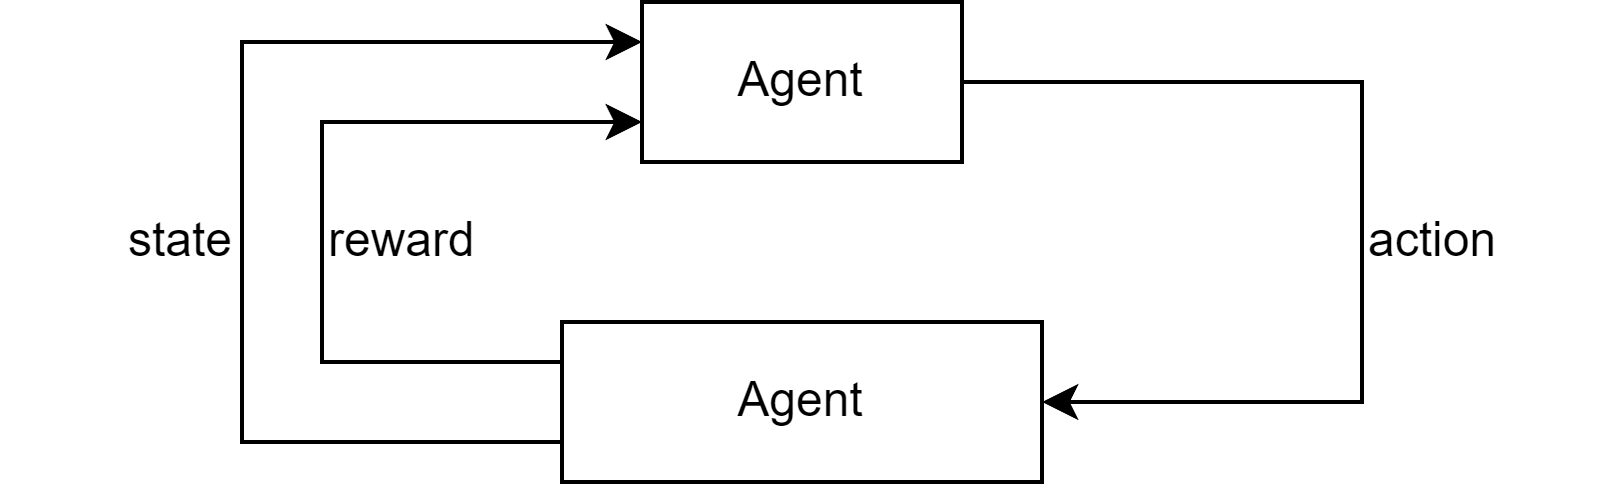
\includegraphics[width=0.75\linewidth]{images/rl.png}
    \caption{Agent-environment interface}
\end{figure}
At each discrete time step $t = 0, 1, 2, K$, the agent and the environment interact according to the following cycle:
\begin{enumerate}
    \item The agent first observes the current state $S_t \in \mathcal{S}$, then selects an action $A_t \in \mathcal{A}(S_t)$ based on that state.
    \item The environment provides a reward $R_{t+1} \in \mathcal{R}$, and the agent's action causes the environment to transition to the next state $S_{t+1} \in \mathcal{S}$.
\end{enumerate}
\begin{figure}[H]
    \centering
    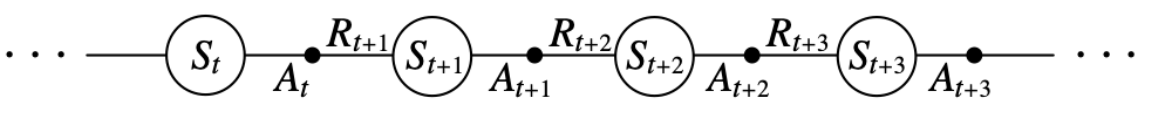
\includegraphics[width=0.75\linewidth]{images/rl1.png}
    \caption{Agent-environment interface}
\end{figure}